% !TEX root = ../paper.tex

\section{Design}

The priority queue implementation by \citeauthor{calciu_adaptive_2014} exports the two necessary operations \texttt{add()} and \texttt{removeMin()}. It is based on a skiplist which is split into two parts as it can be seen in figure~\ref{fig:pqe}. The elements in the skiplist are buckets having associated keys accessible via \texttt{bucket.key}. \texttt{RemoveMin()} and \texttt{add()} operations with small keys are served by the sequential part, while \texttt{add()} operations with keys over a certain threshold are executed on the parallel part. The last element of the sequential part is referred to as \texttt{lastSeq}.

\begin{figure}[htb]
	\centering
	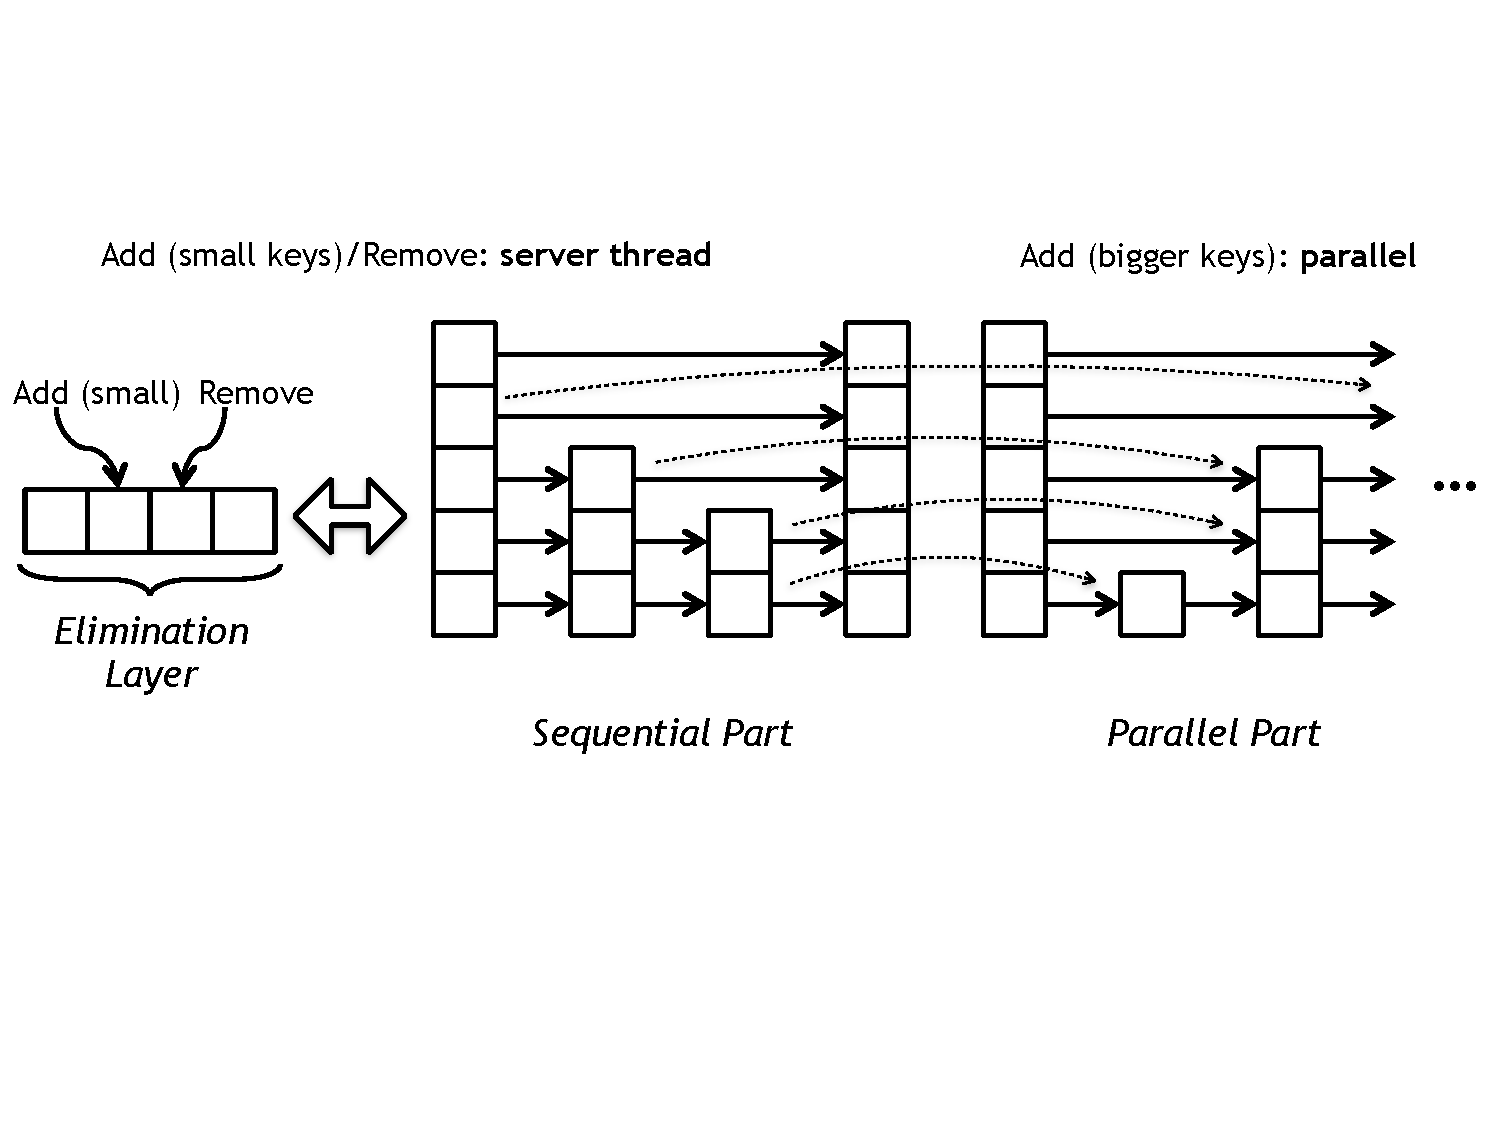
\includegraphics[width=0.9\textwidth]{graphics/pqe.pdf}
	\caption{Skiplist design \cite{calciu_adaptive_2014}.}
	\label{fig:pqe}
\end{figure}

\paragraph{Add()}

A thread executing \texttt{add($v$)} on the priority queue decides whether to insert the element concurrently into the parallel part if $v > \texttt{lastseq.key}$. Otherwise, the element is put into the elimination array. If the element becomes eligible for elimination ($v < \texttt{minValue}$) the operation can eliminate with any \texttt{removeMin()} occurring, otherwise the operation will be executed by the server thread.

\paragraph{RemoveMin()}

\subsection{Elimination and Combining}

\subsubsection{Elimination Array Transitions}

\begin{figure}[htb]
	\centering
	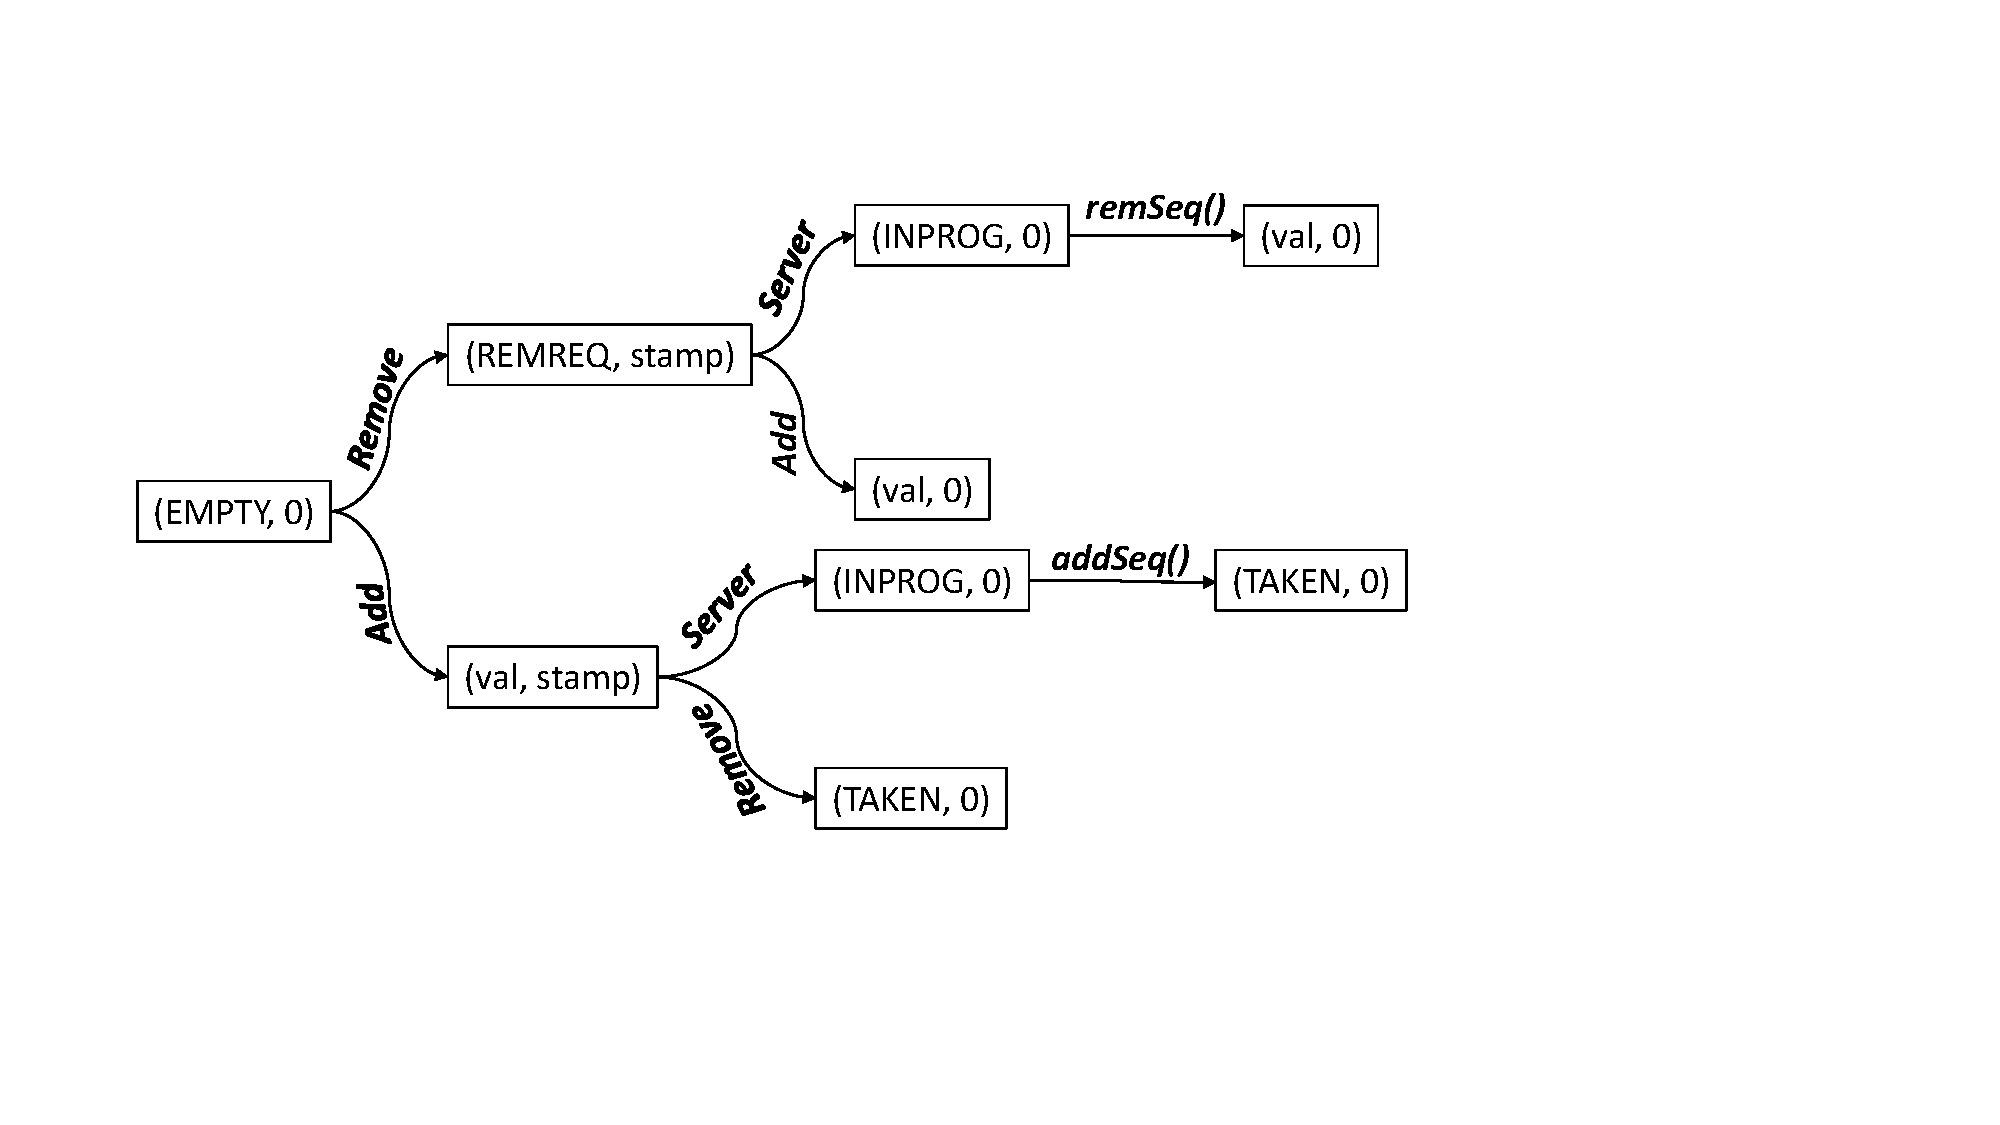
\includegraphics[width=0.9\textwidth]{graphics/combining-state.pdf}
	\caption{\cite{calciu_adaptive_2014}}
	\label{fig:combining-state}
\end{figure}

\subsubsection{Server Thread}

\subsection{Skiplist Operations}

\subsubsection{Sequential Part Operations}

\paragraph{addSeq()}

\paragraph{moveHead()}

\paragraph{chopHead()}

\subsubsection{Parallel Part Operations}

\paragraph{addPar()}

\subsection{Hardware Transactions}

\subsubsection{Head-Moving Operations}

\subsubsection{addPar()}
